
\begin{figure}
\centering
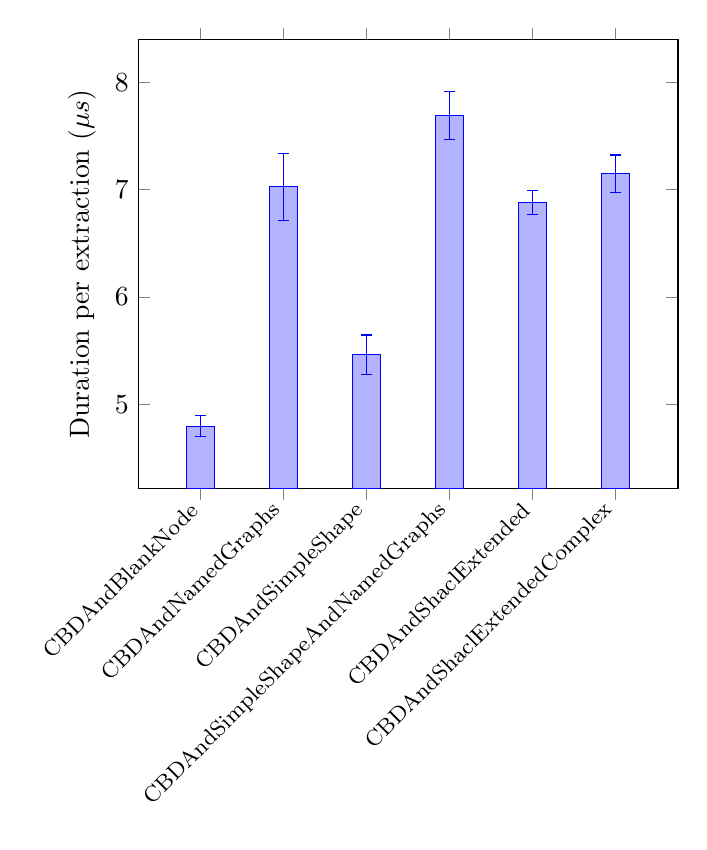
\begin{tikzpicture}
        \begin{axis}[
            ybar,
            enlargelimits=0.15,
            legend style={at={(0.5,-0.15)},
            anchor=north,legend columns=-1},
            ylabel={Duration per extraction ($\mu s$)},
            symbolic x coords={CBDAndBlankNode,CBDAndNamedGraphs,CBDAndSimpleShape,CBDAndSimpleShapeAndNamedGraphs,CBDAndShaclExtended,CBDAndShaclExtendedComplex},
            xtick=data,
            x tick label style={font=\footnotesize,rotate=45, anchor=east},
            nodes near coords align={horizontal},
        ]
            \addplot+[
                error bars/.cd,
                y dir=both,
                y explicit
            ] coordinates {
         (CBDAndBlankNode, 4.797509364622769) +- (0, 0.0958380305767924)
         (CBDAndNamedGraphs, 7.025067210009044) +- (0, 0.3138371070088579)
         (CBDAndSimpleShape, 5.459865414643892) +- (0, 0.18596088787283932)
         (CBDAndSimpleShapeAndNamedGraphs, 7.6894902082499) +- (0, 0.2236745653527336)
         (CBDAndShaclExtended, 6.880947935007133) +- (0, 0.11058598538681243)
         (CBDAndShaclExtendedComplex, 7.147677284904611) +- (0, 0.1737624622779607)

             };
        \end{axis}
    \end{tikzpicture}
    \caption{Graph depicting performance of inband extraction algorithm}
\end{figure}
